\chapter{Methods Critique}
\label{ch:critique}

% SOURCE OF TRUTH: thesis-pack/09-method/EVALUATION_PROTOCOL_V2.md
% (= PREREGISTRATION Amendment 16, 2026-09-22), plus RESULTS sec.6.7 and 6.8,
% the Gate 0 evidence in thesis-pack/11-results/data/discrimination-*.md, and
% the v2 instruments in thesis-pack/11-results/data/v2.md.
%
% TONE RULE. No hedging and no self-flagellation. State the defect, state the
% evidence, state the gate that catches it, state what stands.

This chapter reads the results back against the protocol that produced them.
It exists because the protocol, applied to its own data, found that its primary
arm could not have answered the question it was built for. That finding is
reported here as a result in its own right. A protocol that detects a
degenerate treatment with its own negative control, and then specifies the gate
that would have caught it, has done its job.

The chapter does not repeat the numbers of Chapter~\ref{ch:results}. It points
to them and adds only what is new: the treatment-validity gate and its
evidence, the regret against a null policy, the alternative explanations that
were ruled out, and the position taken on each declared limitation.

Everything in Sections~\ref{sec:crit:gate0} to~\ref{sec:crit:mechanism} was
designed after the evaluation data had been seen. It is registered as
Protocol~v2 in Amendment~16, and under the pre-registration's own rules it is
exploratory without exception. It changes the \emph{name} of what the first
protocol measured. It does not change a single number, and it does not change
the sign of the result.

One boundary holds for the whole chapter. No scenario in this thesis ever
\emph{required} adaptation. RQ1 is therefore answered as ``did the agentic
architecture win here'', not ``can it ever win''.

% =====================================================================
\section{The Defect}
\label{sec:crit:defect}

The novel arm was built to test H2: does the agentic system recover better than
a scripted workflow when a disruption arrives that the workflow has no branch
for? On that arm the workflow baseline scored $S = 1.000$ in all 50 of its
runs. That perfect score is not a recovery. It is an \emph{invariance}, and the
scenario design guaranteed it before any model was chosen.

The reason is in how the scenarios are written. Every event in every one of the
fourteen scenario files is an envelope of the form \texttt{\{at, send\}}: at a
given time, send a given message. No scenario event changes the declared world
state, that is the \code{world}, \code{sensing} or \code{hazard} blocks. The
disruption exists as text in an inbox and nowhere else. When SC1 reports a
partial capacity loss, SC1 keeps declaring 60 beds. When bus-1 is suspended,
bus-1 keeps its seats.

So the baseline's physical plan is not touched by the disruption. It drives
60.63 bus-km on the undisrupted \code{closed_loop} and 60.63 bus-km on each of
the five novel disruptions (Section~\ref{sec:res:responsetime}). Not one
kilometre moves.

The protocol's own negative control confirms this. The no-replan control of
Section~\ref{sec:eval:noreplan} is the doctrine baseline with re-planning
switched off, so it ignores every disruption. Run against the scored scenarios,
it commits byte-identical orders and scores the identical level on all five
novel files and on \code{closed_loop}.

On the novel arm, then, \textbf{ignoring the disruption is an optimal policy}.
A test in which doing nothing scores at the ceiling cannot produce evidence for
or against an adaptability hypothesis, in either direction. The agentic
system's only route to a non-negative risk difference was to also do nothing,
and doing nothing is exactly what an agentic architecture is built not to do.

The first protocol knew the mechanism and wrote it down. As
Section~\ref{sec:eval:noreplan} quotes, it stated that on every scored scenario
the control ``cannot differ from the doctrine in outcome, by construction''.
It used that note as the reason to read the negative control on a separate
fixture. The error was not concealment. The error was that the gate's guarantee
was never required to hold on the files where the hypotheses were actually
read.

% =====================================================================
\section{Gate 0: Treatment Validity}
\label{sec:crit:gate0}

Protocol~v2 adds a gate that is read before Gates 1 to 3, and read per
scenario rather than per system:

\begin{quote}
A scenario is admitted to a confirmatory adaptability arm only if a system
that ignores its disruption scores strictly worse on it than one that
responds.
\end{quote}

A scenario that fails Gate~0 may still be run and reported. It is then a
legitimate test of \emph{base execution}. But it may not carry an adaptability
claim, and no risk difference computed on it may be described as evidence about
re-planning. The gate is cheap. It costs two runs of the control per scenario
and reuses the no-replan machinery the first protocol already built.

A disruption is \emph{binding} when three conditions hold. Each one isolates a
different way a scenario can fail to test what it was written to test.

\begin{description}
\item[D1, state-mutating.] The disruption changes declared world state, not
  only an inbox. A purely informational disruption can still bind in principle,
  if acting on the information is required to succeed. But this cannot be
  assumed.
\item[D2, order-binding.] The null policy does not commit the same order
  sequence as the responding policy. If the orders are byte-identical, no
  downstream instrument can tell the two apart, whatever it measures.
\item[D3, outcome-binding.] The null policy scores a strictly lower outcome.
  D2 without D3 means the plans really differ, but the scoring function cannot
  see it.
\end{description}

A fourth condition applies to the scenario \emph{set}, not to each scenario.
\textbf{D4, recoverable:} at least one policy must reach the feasibility
ceiling. A disruption that no policy can recover from measures the hazard, not
the coordinator.

Table~\ref{tab:crit:gate0} is the evidence. It runs the doctrine baseline and
the no-replan control side by side on the fixture and on all seven scored
scenarios. Both variants are scored without a clean-run reference, so both are
capped at level 3. The comparison is between the two variants, not against the
campaign's level 4.

\begin{table}[htbp]
\centering
\caption[Gate 0 evidence: the no-replan control on the scored scenarios]{Gate~0
evidence. The doctrine baseline against the no-replan control, which ignores
every disruption. $L$ is the level, capped at 3 here, with completeness in
brackets. Only the fixture discriminates. Exploratory.}
\label{tab:crit:gate0}
\scriptsize
\setlength{\tabcolsep}{3.5pt}
\begin{tabular}{lccccccc}
\toprule
 & & orders & \multicolumn{2}{c}{level $L$ (C)} & \multicolumn{2}{c}{bus-km} & discri- \\
\cmidrule(lr){4-5}\cmidrule(lr){6-7}
Scenario & world & identical & doctrine & no-replan & doctrine & no-replan & minates \\
\midrule
\emph{fixture:} \code{shelter_closure} & yes & no & 3 (1.0) & 0 (0.0) & 83.12 & 38.14 & \textbf{yes} \\
\midrule
\code{medical_emergency_in_flight} & yes & yes & 3 (1.0) & 3 (1.0) & 60.63 & 60.63 & no \\
\code{unverified_persons_report} & yes & yes & 3 (1.0) & 3 (1.0) & 60.63 & 60.63 & no \\
\code{conflicting_evacuation_orders} & yes & yes & 3 (1.0) & 3 (1.0) & 60.63 & 60.63 & no \\
\code{bus1_suspension_capacity_reduction} & yes & yes & 3 (1.0) & 3 (1.0) & 60.63 & 60.63 & no \\
\code{sc1_partial_capacity_loss} & yes & yes & 3 (1.0) & 3 (1.0) & 60.63 & 60.63 & no \\
\code{closed_loop} & yes & yes & 3 (1.0) & 3 (1.0) & 60.63 & 60.63 & no \\
\code{road_closure} & no & no & 3 (1.0) & 3 (1.0) & 83.12 & 38.14 & no \\
\bottomrule
\end{tabular}
\end{table}

Every scored row reads \emph{discriminates: no}. On the five novel
disruptions the two variants are indistinguishable at every level of the
instrument: same orders, same kilometres, same level. They fail all three
conditions.

\code{road_closure} fails in a different way, and it is worth reading
closely. It is the one scored file where the null policy commits
\emph{different} orders, 83.1 km against 38.1 km. So it passes D2. But the
scenario declares no \code{world}, so dropoffs are injected by the scenario
rather than earned by the plan, and completeness ties whatever was ordered. The
disruption binds the orders and still does not bind the outcome. It fails on
D3.

\code{closed_loop} carries no disruption, so Gate~0 does not apply to it. It
is listed for completeness, and its result is not affected.

\textbf{Zero of the six disruption scenarios are admitted.} The one scenario in
the repository that passes is the shelter-closure fixture, where the doctrine
reaches level 3 and the null policy level 0. That is exactly why the first
protocol chose it as the discrimination fixture, and it is exactly the property
the evaluation set lacks.

The contribution this chapter claims is the gate itself. The first protocol had
a negative control and read it on a fixture. Protocol~v2 requires that a
disruption pass the negative control \emph{before} it can be scored as a
disruption at all. That turns a check on the instrument into a check on every
treatment. How to write a scenario that passes it is a design question, and
Section~\ref{sec:design:gate0} carries it.

% =====================================================================
\section{What Is Withdrawn and What Stands}
\label{sec:crit:withdrawn}

This is where an examiner will push, so the boundary is drawn precisely.

\subsection{Withdrawn}

\paragraph{H2's verdict, as a statement about adaptability.} The sentence
``the workflow baseline recovers better from unanticipated disruption'' is not
supported, and this design could not have supported it. The baseline did not
recover. It was not disturbed. No sentence in this thesis describes the
baseline as having adapted, recovered or re-planned better.

\paragraph{H1's verdict on \texttt{road\_closure}.} The same reason applies at one
remove. The disruption changes the orders but not the outcome
(Section~\ref{sec:crit:gate0}), so a survival comparison on it says nothing
about re-planning.

\paragraph{The scope is wider than the novel arm.} Gate~0 fails on all seven
scored scenarios, not only the five novel ones. That is broader than the
question the withdrawal started from, and it is what the evidence supports.

\subsection{Not Replaced by an Agentic Win}

The withdrawal cuts one way only. The baseline's score is uninformative about
adaptation. That does not make the agentic score look better. The agentic
models lost between 10 and 27 residents per 100 on scenarios where the correct
plan required no change at all. The scenario design explains why the
\emph{baseline's} score is uninformative. It does not explain why the
\emph{agentic} score is low.

\subsection{Standing, Unchanged}

\begin{itemize}
\item \textbf{Every number.} Nothing in Protocol~v2 regenerates the scores.
  $S$, every risk difference, every recovery level and all 27 Gate~1 verdicts
  are byte-identical before and after.
\item \textbf{The agentic deficit.} It is real, it is large, and the next
  subsection makes it sharper, not softer.
\item \textbf{\code{closed_loop}.} It has no disruption, so the question there
  is base execution, not adaptation. glm-5.2's non-inferiority pass on it
  stands in full.
\item \textbf{The decision rubric.} It reads the structure of decisions, not
  outcomes, and does not depend on the null policy's score. Its split verdict
  stands as Section~\ref{sec:res:quality} reports it: parity on five criteria,
  a baseline advantage on five.
\end{itemize}

\subsection{Regret Against the Null Policy}
\label{sec:crit:regret}

The first protocol compared the two systems only with each other. It lacked the
quantity that would have exposed the problem: how each system scores against
doing nothing. Protocol~v2 adds it as null-policy regret,
\begin{equation}
R = S_{\text{system}} - S_{\text{null}},
\label{eq:crit:regret}
\end{equation}
measured per run, on survival, against the no-replan control. $R > 0$ means
responding helped. $R = 0$ means responding bought nothing. $R < 0$ means the
system harmed itself by responding. Survival is used instead of level because
the null-policy runs are capped at level 3 while scored runs reach level 4, so
a level difference would be an artifact of the cap.

\begin{table}[htbp]
\centering
\caption[Null-policy regret on the novel arm]{Null-policy regret over the five
novel disruptions, 50 runs per row. Exploratory.}
\label{tab:crit:regret}
\small
\begin{tabular}{lcccc}
\toprule
System and model & mean regret & helped & neutral & harmed \\
\midrule
workflow baseline & $+0.000$ & 0 & \textbf{50} & 0 \\
agentic / qwen3.5 & $-0.100$ & 3 & 30 & 17 \\
agentic / glm-5.2 & $-0.160$ & 0 & 34 & 16 \\
agentic / deepseek-v4-pro & $-0.273$ & 0 & 15 & 35 \\
\bottomrule
\end{tabular}
\end{table}

\begin{figure}[htbp]
\centering
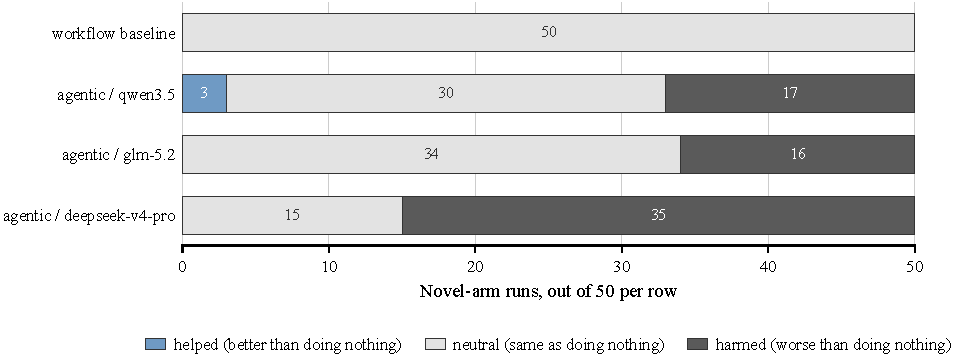
\includegraphics[width=\textwidth]{pics/critique-regret.pdf}
\caption[Null-policy regret per run]{Each novel-arm run against the null
policy, which ignores the disruption. The baseline ties it in every run. The
agentic models tie it or do worse, and three runs of 150 do better.
Exploratory. Drawn from \texttt{data/null\_policy\_regret.csv}.}
\label{fig:crit:regret}
\end{figure}

Table~\ref{tab:crit:regret} and Figure~\ref{fig:crit:regret} need to be read
together, because the two systems say different things.

\textbf{The baseline's regret is exactly zero in all 50 runs.} It gained
nothing by responding. Its response to each disruption changed no order and no
kilometre. The headline ``the workflow baseline beats the agentic system on
resident survival in every disruption tested'' is arithmetically true. It
describes a contest in which one party did not have to compete.

\textbf{The agentic regret is negative everywhere.} No cell is positive on
average; the mean is negative in all 15 model and disruption cells. Of 150
runs, three improved on the null policy, 79 tied it, and \textbf{68 came out
worse than doing nothing}. This is a harsher statement than the first
protocol's. That protocol said the agentic system lost to a better system.
Regret says it lost to inaction. A negative regret is a self-inflicted loss,
and it cannot be blamed on the scenario being hard.

The capability ordering of Section~\ref{sec:res:models} survives intact:
deepseek-v4-pro at $-0.273$, glm-5.2 at $-0.160$, qwen3.5 at $-0.100$. Under
regret it reads as how much damage the response did, not as how far behind the
baseline each model fell.

% =====================================================================
\section{The Mechanism, Corrected by Measurement}
\label{sec:crit:mechanism}

The first write-up explained the agentic deficit in prose. It said the agents
lost residents ``at the handshakes'': a driver's completion call that times out
and is never retried, a facility query that is never answered. That diagnosis
was plausible, and it was never measured. Protocol~v2 measured it, and the
measurement did not support it.

\subsection{What the Instruments Showed}

Chapter~\ref{ch:results} already reports the numbers, so they are only
collected here. Handshake closure is 0.938 over 1\,932 addressed requests, and
the three highest-volume handshakes close at 0.947, 0.970 and 0.997
(Section~\ref{sec:res:loss:handshakes}). The dominant loss mechanism is
residents who were never dispatched, with $r = -0.745$ against survival. The
loss is quantised at whole bus-loads (Figure~\ref{fig:res:delivery}). And the
full-delivery rate falls from 90\% at the minimum number of plan revisions to
32\% at six or more (Table~\ref{tab:res:commitment}).

The message layer did its job. The failure is in what the agents decided to
move, not in whether their messages arrived.

\subsection{The Alternatives That Were Ruled Out}

A diagnosis is only as strong as the alternatives it eliminates.
Table~\ref{tab:crit:ruledout} lists every candidate cause that was tested
against the 150 agentic novel runs, and the verdict on each.

\begin{table}[htbp]
\centering
\caption[Candidate causes of the agentic loss, and the verdict on each]{Candidate
causes of the agentic loss, tested against the 150 agentic novel runs.
Exploratory.}
\label{tab:crit:ruledout}
\small
\begin{tabularx}{\textwidth}{>{\raggedright\arraybackslash}p{5.2cm}>{\raggedright\arraybackslash}X}
\toprule
Candidate cause & Verdict \\
\midrule
The agents were told the wrong population & \textbf{No.} 100 residents were correctly reported in 150 of 150 runs. \\
The database message layer failed & \textbf{No.} Handshake closure is 0.938. \\
Too few missions dispatched, or the reserve bus held back & \textbf{No.} About 2.3 dispatch orders in failing and successful runs alike. Bus-2 was used in every run. \\
The scorer's arrival de-duplication removed real deliveries & \textbf{No.} De-duplicated arrival sums track sheltered residents. \\
Drivers over-claimed their headcount & \textbf{No.} 54 discrepancy rows, with $r = +0.061$ against $S$. \\
The run simply ran out of clock & \textbf{Mostly no.} Only 5 of the 19 total-loss runs recorded a dropoff after 12:00. \\
\bottomrule
\end{tabularx}
\end{table}

What is left is a \textbf{commitment failure, not a comprehension failure}. The
agents understood the disruption, addressed the right parties and had their
messages answered. What they could not do was carry one committed plan through
to delivery. Legs were re-planned while in flight, and the coordinator often
could not establish whether a leg had finished. The coordinator's own abort
messages name this directly, for example ``bus-2 reassigned to immediate
emergency dispatch, original mission never delivered'' and ``zero deliveries
across 8 transport plan revisions''.

This cuts against the architecture's own claim. Re-planning on disruption is
the capability the agentic design advertises. On these scenarios the correct
number of re-plans was zero.

\subsection{What Is Not Established}

The causal direction is open, and this thesis does not claim it. A run that is
going badly re-plans \emph{because} it is going badly. Nothing in an
observational arm separates that from re-planning causing the loss.

The abort messages show how much this matters. Each abort was classified by its
stated reason. Of 108 aborts, 57 (52.8\%) are explicit stand-downs after a
failure, 14 (13.0\%) are clearly started by a re-plan, and 37 (34.3\%) are
other. The order of classification is important. A stand-down message often
names the re-dispatch attempts that came before it, for example ``Hochbahn
unresponsive to 3 redispatch requests over 18 min''. That message is a
\emph{consequence} of the failure, not a re-plan that caused it. So the
failure response is tested first. Testing for churn first would misclassify
these messages and inflate a causal reading the design cannot support.

The experiment that would settle the direction is a
\textbf{commitment-constrained variant}: cap the number of re-plans, or forbid
cancelling a leg that is already in flight, and run it on the same scenarios
with the same models. It is one campaign and needs no new scenarios. It is
future work, not a defect of this study, and it is the most valuable follow-up
this analysis produces.

\subsection{A Lesson From Measuring Handshakes}

Measuring closure was harder than it looks, and three reading rules carry the
instrument. Each one silently zeroes a whole handshake type if it is dropped.
Agent ids are written two ways, so a driver addressed as
\code{agent-bus-driver-1} signs as \code{bus-driver-1}; exact string matching
reports closure as 0.50 instead of 0.94. The message \code{confirm_dropoff} has
two jobs: to a shelter it asks for intake, to Hochbahn it only reports progress
and expects no answer. And no clock in the log orders two agents' rows, because
each recipient stamps its own simulated time. Closure is therefore defined as a
matching between requests and replies, which is stable under any ordering, and
\textbf{no reply latency is reported at all}. The data cannot support a latency
claim.

% =====================================================================
\section{The Pre-Registered Primary Was Underpowered by Construction}
\label{sec:crit:power}

Two separate things are reported here, and they should not be merged.

\paragraph{A timing deviation.} The pre-registration named a Clopper-Pearson
interval, a scenario-level sign test and a Holm-Bonferroni correction as the
primary test for H2. None of the three existed in the code when the H2 verdict
was first written. They were implemented afterwards, once the result was known
(Amendment~15). Under the pre-registration's own rules that analysis is
exploratory. It agrees with the verdict it was checking
(Section~\ref{sec:res:novel:prereg}), which does not excuse the timing.

\paragraph{A design finding.} This is the more interesting one. At $k = 10$ the
registered aggregation could not reach conventional significance however the
data fell. A two-sided exact sign test on five scenarios cannot return a $p$
below 0.0625, even when every scenario points the same way. Ties push the floor
higher. qwen3.5 and glm-5.2 each tie two scenarios, which leaves three untied
observations and a floor of 0.250. Table~\ref{tab:res:signtest} shows that
both models sit exactly at the smallest $p$ their data could have produced.
The design would not have detected a moderate effect even if one had existed.

This is a finding about pre-registered analysis plans, not an apology for this
one. A registered primary that cannot reach significance is not a test.
Protocol~v2 draws three consequences from it:

\begin{enumerate}
\item The registered primary must be one the design can detect. The paired
  risk difference, which is continuous and far more efficient, becomes
  primary. The sign test becomes a supporting robustness check.
\item The minimum detectable effect is declared before any run. If it exceeds
  the registered margin, either $k$ rises or the claim is dropped, before data
  collection and not after.
\item Cells that fail Gate~0 are excluded from confirmatory arms by rule, not by
  judgement and not after the result is known.
\end{enumerate}

% =====================================================================
\section{The Cut-Point Sensitivity Analysis}
\label{sec:crit:sensitivity}

The protocol made a sensitivity analysis on the level cut points a
precondition on the headline. The first write-up did not contain it. The
summary said it must be reported, but printed no table, and the reporting
script never read the field. The check existed on paper and not in code.

It is now emitted, and it supports the headline (Section~\ref{sec:res:sensitivity}).
With the cut moved to 0.40, 0.50 and 0.60, every cell in the three full novel
arms keeps its median level except one, deepseek on
\code{unverified_persons_report}, which moves from 2.0 to 1.5 at 0.60. No
ordering between the agentic system and the baseline moves anywhere in the
range. The lesson is procedural: a precondition that a report asserts but does
not compute is not a precondition. It should fail the build.

% =====================================================================
\section{Limitations Declared, With the Position Taken on Each}
\label{sec:crit:limitations}

Table~\ref{tab:crit:limits} lists the six limitations that came out of
executing the design. Each is a position, not an open question, and none
requires further work before submission. The limitations declared before the
evaluation are in Table~\ref{tab:eval:scope}.

\begin{table}[htbp]
\centering
\caption{Declared limitations and the position taken on each.}
\label{tab:crit:limits}
\small
\begin{tabularx}{\textwidth}{>{\raggedright\arraybackslash}p{4.4cm}>{\raggedright\arraybackslash}X}
\toprule
Limitation & Position \\
\midrule
The novel arm was not a valid adaptability test &
Declared, and claimed as the methods contribution. The protocol's own negative
control shows the null policy at the ceiling on every scored scenario, so H2
could not have resolved in either direction (Section~\ref{sec:crit:gate0}). \\
\addlinespace
The causal direction of plan churn is open &
Future work, not a defect. Plan revisions track survival, but most aborts are
stand-downs after a failure. The commitment-constrained variant is the
experiment that would settle it (Section~\ref{sec:crit:mechanism}). \\
\addlinespace
Parity deviation 7 was still open when the campaign ran &
Closed by written re-argument, which the protocol's gate allows. The
deviation runs against the baseline, so it cannot explain a baseline win. It
could only have understated the margin (Section~\ref{sec:val:dev7}). \\
\addlinespace
42 of 87 doctrine elements have no page citation &
A limitation on the claim that the baseline is doctrine-grounded, and on
nothing else. It affects no number. 45 of 87 elements are cited to a page, the
rest are asserted by the author. \\
\addlinespace
Only one time scale ran (8.4) &
H4 was not tested. No crossover, trend or scale-dependence claim is made
anywhere. The evaluation is finished, so this is permanent. \\
\addlinespace
The registered H2 primary was implemented late &
Disclosed and labelled exploratory. Reported as a methods finding: the
registered primary was underpowered by construction
(Section~\ref{sec:crit:power}). \\
\bottomrule
\end{tabularx}
\end{table}

A second group of caveats applies to individual tables rather than to the
design. Each is disclosed where its effect is visible, and they are collected
here so that none is missed.

\begin{itemize}
\item \textbf{Levels are comparable only across the three full arms.} Partial
  model series have no clean-run reference and are capped at level 3. They are
  compared on $S$ only (Section~\ref{sec:res:models:levelcap}).
\item \textbf{Six runs shelter more residents than the ceiling admits.} The cap
  is applied at the reporting layer, not in the scorer
  (Section~\ref{sec:res:integrity:ceiling}).
\item \textbf{The novel arm's third model changed four times} after data were
  seen, so that arm's model set is exploratory
  (Section~\ref{sec:res:models:churn}).
\item \textbf{Two runs executed on a dirty working tree}, with routing changes
  that were committed later. The exclusion rules do not admit this as a reason,
  so they are kept and disclosed.
\item \textbf{28 of 168 agentic novel runs did not quiesce.} The outcome was
  decided in all of them, but a final message may be missing from the log.
\item \textbf{The cloud model tags are not version-frozen}, so no digest pins
  these results.
\item \textbf{Three asymmetries favour the baseline}: the reserve-bus
  serialisation on the agentic side, a fallback playbook that mis-frames two
  message types for the agents, and the anchor of a replacement bus leg.
  Chapter~\ref{ch:validity} states each with its direction
  (Sections~\ref{sec:val:extra} and~\ref{sec:val:reserve}). Each runs in the
  baseline's favour, so none of them can explain the agentic deficit away.
\end{itemize}

% =====================================================================
\section{What This Protocol Still Does Not Measure}
\label{sec:crit:scope}

Protocol~v2 removes nothing from the scope table of the first protocol
(Table~\ref{tab:eval:scope}). Table~\ref{tab:crit:scope} adds the limits that
v2 introduces or inherits.

\begin{table}[htbp]
\centering
\caption{What Protocol~v2 still does not measure.}
\label{tab:crit:scope}
\small
\begin{tabularx}{\textwidth}{>{\raggedright\arraybackslash}p{5.2cm}>{\raggedright\arraybackslash}X}
\toprule
Not measured & Why \\
\midrule
Whether the agentic architecture wins on a scenario that passes Gate~0 &
No such scenario has been run. Protocol~v2 makes the question askable. It does
not answer it, and nothing here licenses a claim about what would happen. \\
\addlinespace
Reply latency & No clock in the log orders two agents' rows. Closure is
measured, lag is not. \\
\addlinespace
Whether a reply was correct & Closure asks whether an answer came back, never
whether it was right. A shelter that confirms an intake it cannot hold still
counts as closed. \\
\addlinespace
Whether over-budget runs would do better at a slower clock & Only one time
scale was run. H4 was not tested and now cannot be. \\
\addlinespace
Any confirmatory claim & Every v2 instrument was written after the data were
seen. \\
\addlinespace
The baseline's coordination cost under a binding disruption & Its 13 messages
per run were measured on scenarios that asked for no re-planning. A scenario
that did would raise that number by an unknown amount. \\
\bottomrule
\end{tabularx}
\end{table}

Taken together, the chapter leaves six points for the reader.

\begin{enumerate}
\item The comparison was run on scenarios where the baseline could not lose.
  Its perfect survival is invariance, not recovery, and the no-replan control
  shows this on every scored file.
\item The agentic deficit is nonetheless real, and it is now measured more
  sharply. Against the null policy its regret is negative in every cell, and
  68 of 150 runs came out worse than doing nothing.
\item The mechanism is not the one first named. The message layer closes 94\%
  of addressed requests. The loss is dominated by residents never dispatched.
\item It is a commitment failure, not a comprehension failure. The loss comes
  in whole bus-loads, and full delivery falls from 90\% to 32\% as plan
  revisions rise. The causal direction is not established.
\item The architecture's cost is an order of magnitude higher and is now
  printed (Section~\ref{sec:res:responsetime}).
\item Whether that cost ever buys anything is untested, because no scenario in
  this thesis ever required it to. A campaign on scenarios that pass Gate~0 is
  the experiment that would find out.
\end{enumerate}
